\documentclass[draft,12pt,headsepline,footsepline,paper=letter]{scrreprt}
\pagestyle{headings}

\usepackage[utf8]{inputenc}
\usepackage[T1]{fontenc}
\def\spanishoptions{es-noquoting,es-nolists,mexico-com}
\usepackage[spanish]{babel}

\usepackage{makeidx}
\makeindex

\usepackage[nonumberlist]{glossaries}
\makeglossaries

\usepackage[final]{graphicx}
\DeclareGraphicsExtensions{.pdf,.png,.jpg}
\graphicspath{{media/}}
\usepackage{rotating}

\usepackage{scrhack}

\usepackage{natbib}
\usepackage{amsmath,amssymb, bm}
\usepackage{enumerate}
\usepackage{ragged2e}
\usepackage{nameref}

\usepackage{setspace}
\onehalfspacing
\frenchspacing
\recalctypearea

\usepackage{marginnote}
% \usepackage{hyperref}

\setlength{\parindent}{0.25in}
\renewenvironment{quotation}{\list{}{\leftmargin=0.25in}\item[]}{\endlist}
\newcommand{\BigO}{\ensuremath{\mathcal{O}}}% big-O notation/symbol
\addto\captionsspanish{
  \renewcommand\bibname{Referencias}
}
% Glossary
\newglossaryentry{asignatura} {
	   name = asignatura,
    description = {Materia que se enseña en un curso y que forma parte de un programa de estudios}}
\newglossaryentry{aula} {
	   name = aula,
    description = {Sala de un centro de enseñanza donde se imparten clases}}
\newglossaryentry{calendario} {
    name        = calendario,
    description = {Plan ordenado del conjunto de las actividades previstas durante un período}}
\newglossaryentry{calendarizacion} {
           name = calendarización,
    description = {Acción y efecto de calendarizar}}
\newglossaryentry{calendarizar} {
           name = calendarizar,
    description = {Establecer un calendario ordenado de actividades previstas}}
\newglossaryentry{catedra} {
           name = cátedra,
    description = {Aula en la que se enseña una asignatura}}
\newglossaryentry{clase} {
           name = clase,
    description = {Conjunto de escolares o estudiantes de un mismo nivel o que estudian la misma asignatura, y que asisten juntos a las lecciones correspondientes}}
\newglossaryentry{conferenciante} {
           name = conferenciante,
    description = {Persona que pronuncia una conferencia}}
\newglossaryentry{curriculo} {
           name = currículo,
    description = {Plan de estudios}}
\newglossaryentry{curso} {
           name = curso,
    description = {Conjunto de lecciones o clases sobre una materia que está estructurada y sigue un programa, especialmente dentro de un plan de estudios}}
\newglossaryentry{educacional} {
           name = educacional,
    description = {Perteneciente o relativo a la educación}}
\newglossaryentry{escuela} {
           name = escuela,
    description = {Institución o establecimiento destinados a enseñar determinadas materias especializadas}}
\newglossaryentry{factible} {
           name = factible,
    description = {Que se puede hacer}}
\newglossaryentry{horario} {
           name = horario,
    description = {Distribución de las horas en que se realiza una actividad o trabajo o se presta un servicio}}
\newglossaryentry{leccion} {
           name = lección,
    description = {Sesión docente en la que el profesor de una materia imparte un conjunto articulado de conocimientos}}
\newglossaryentry{limitacion} {
           name = limitación,
    description = {Circunstancia o condición de algo o de alguien que limita, impide o dificulta su desarrollo}}
\newglossaryentry{prevalente} {
           name = prevalente,
    description = {Que prevalece o sobresale}}
\newglossaryentry{programacion} {
           name = programación,
    description = {Acción de programar}}
\newglossaryentry{programar} {
           name = programar,
    description = {Establecer o planificar el programa de una serie de actividades}}
\newglossaryentry{turno} {
           name = turno,
    description = {Conjunto de trabajadores que desempeñan su actividad al mismo tiempo, según un orden establecido previamente}}
\newglossaryentry{revision bibliografica}{
          name = revisión bibliográfica,
   description = {La revisión bibliográfica comprende todas las actividades relacionadas con la búsqueda de información escrita sobre un tema acotado previamente y sobre el cual, se reúne y discute críticamente, toda la información recuperada y utilizada}}
\newglossaryentry{planeacion}{
          name = planeación,
   description = {Mex. Planificación}}
\newglossaryentry{procedimental}{
          name = procedimental,
   description = {Del procedimiento o relacionado con él:la exigencia de total y absoluta formalidad procedimental}}
\newglossaryentry{precedencia}{
          name = precedencia,
   description = {Circunstancia de preceder a una cosa o persona en el tiempo o en el espacio o de tener más importancia que otra persona o cosa:la precedencia de un acontecimiento sobre otro}}
\newglossaryentry{patron}{
          name = patrón,
   description = {Cosa que se toma como modelo o punto de referencia para medir o valorar otras de la misma especie:patrón de conducta; la alegría es imponderable, pues no existe ningún patrón para medirla}}

\newacronym[longplural=Frames per Second]{fpsLabel} {FPS}{Frame per Second}


\begin{document}

\title{Calendarización en instituciones educacionales}
\author{Héctor Arciga}
\date{\today}

\maketitle

\begin{abstract}
Abstract
\end{abstract}

\begin{spacing}{1}
\tableofcontents
\glsaddall
\printglossaries
\listoffigures
\listoftables
\end{spacing}

\chapter{Introducción}

\section{Antecedentes y motivación}

Las instituciones educativas como factor de cambio social juegan un papel importante en el amoldamiento del individuo, en particular cuando la formación es obligatoria y a modo del Estado. Es bajo estas condiciones que el gestor escolar debe diseñar sus estrategias para alcanzar sus objetivos institucionales.
Si bien el gestor escolar en el sector público no cuenta con el mismo grado de laxitud operativa que su contra-parte en la iniciativa privada, ambos tienen alternativas de acción similares para afectar el desempeño de su institución.
Mucho se ha hablado de maneras para mejorar el nivel educativo en las instituciones educativas desde la inversión de recursos en infraestructura; la capacitación continua de los docentes; el aprovisionamiento gratuito de útiles escolares, uniformes, alimentos; la  inclusión de las nuevas tecnologías informáticas en la pedagogía; mejoras en las condiciones laborales del magisterio;

\section{Objetivos de la investigación}

Esta tesis investiga la problemática de la elaboración de horarios en instituciones docentes y el impacto potencial de su formulación en distintas métricas de desempeño educacional relevantes para el gestor\index{gestor escolar} escolar.
El fin primordial del trabajo es investigar de qué manera puede el gestor escolar hacer uso de estas técnicas, para la consecución de sus estrategias.
Para poder cumplir con esta finalidad, los siguientes objetivos son considerados:
\begin{enumerate}[1]
\item La investigación de las distintas problemáticas en la planificación de horarios en instituciones docentes.
\item Las distintas formulaciones\index{formulación matemática} matemáticas de los problemas de planificación de horarios.
\item Los algoritmos de solución disponibles para este tipo de modelos matemáticos.
\item Los antecedentes históricos de técnicas de optimación aplicados a partir del surgimiento de los ordenadores.
\item La recopilación de las métricas\index{métricas de desempeño} de desempeño educacional relevantes para los gestores escolares.
\item Una investigación de las restricciones más comunes utilizadas en las formulaciones de los problemas de planificación de horarios.
\end{enumerate}

\section{Descripción de la tesis}

Esta tesis consiste de ocho capítulos. El presente capítulo presenta los antecedentes, motivación y objetivos de la investigación. El resto de la tesis está organizada de la siguiente manera:

El Capítulo 2 presenta una visión general de la problemática así como su clasificación en la literatura.

Los preliminares de la calendarización en general aparecen en el Capítulo 3.

En el Capítulo 4 se detallan los modelos matemáticos y los algoritmos existentes para su solución así como una propuesta de un lenguaje en común para la representación de los problemas.

Las restricciones y funciones objetivo más comunes en la literatura se exponen en el Capítulo 5.

El papel del gestor escolar se discute en el Capítulo 6.

En el Capítulo 7 se hace una exposición del tipo de herramientas existentes para la solución de estos problemas así como un listado de algunas opciones de software encontradas.

Por último, en el Capítulo 8 se presenta un resumen del trabajo de investigación, las contribuciones hechas en el mismo, el trabajo futuro y la diseminación de trabajo.

\chapter{Preliminares}
\label{preliminares}

\section{Introducción}
\label{introduccion_preliminares}

Este capítulo es una revisión bibliográfica enfocada en los aspectos fundamentales del área de investigación.
Introduce conceptos primordiales para el estudio del problema general de programación, los elementos que lo componen, su proceso de elaboración, la teoría detrás de los modelos matemáticos, así como la clasificación de los problemas.
El capítulo comprende de 7 secciones. La sección \ref{programacion_elementos} introduce los conceptos de programación\index{programación} y programa\index{programa} así como los elementos involucrados en el proceso\index{programación!proceso} de programación, esclarece términos prevalentes en la literatura y establece la definición de conceptos relevantes. 

\section{La programación y sus elementos} % (fold)
\label{programacion_elementos}

La programación\index{programación} como palabra, forma parte del vocabulario de todos los días —aunque no siempre se tenga una idea clara de su significado–. En realidad, no es la programación en sí lo que es una noción común de la vida diaria, son más bien los programas\index{programa}. Un programa es un plan o documento tangible, tal como el programa de salidas de un autobús o un programa de clases. Un programa señala cuándo debe suceder algún evento\index{evento}; especifíca un plan para el tiempo de ocurrencia de ciertas actividades\index{actividad} y contesta la pregunta, «Si todo va bien, ¿cuándo ocurrirá un evento determinado?» \cite[p.~1]{Baker2009}.

Supóngase que es deseable saber cuándo será servida la cena o cuándo un autobús saldrá a su destino. En estos casos, el evento\index{evento} de interés es la compleción de una actividad\index{actividad} particular —como lo es la preparación de la cena— o el comienzo de una actividad específica —como el viaje en autobús—. Las respuestas a la pregunta «¿cuándo?» usualmente están relacionadas con información de tiempos\index{tiempo}. La cena está programada para ser servida a las 18:00, el autobús está programado para salir a las 8:00. Sin embargo, una respuesta igualmente útil puede ser dada en términos de secuencia\index{secuencia} en lugar de tiempo: es decir, la cena será servida tan pronto como el platillo principal esté horneado, o el autobús partirá a su destino en cuanto su limpieza y mantenimiento sean completados. Por lo tanto, la pregunta «¿cuándo?» puede ser contestada ya sea con información de secuencia o de tiempos obtenida a partir de un programa \citep[p.~1]{Baker2009}.

De manera intuitiva, se puede pensar que la programación\index{programación} es el proceso\index{programación!proceso} de producir un programa\index{programa}, sin embargo rara vez se consideran los detalles que ello conlleva. De hecho, aunque se piense en un programa como algo tangible, el proceso de programación parece no serlo, hasta que es considerado con cierto detenimiento. El problema es comúnmente atacado en dos pasos: secuenciación\index{secuenciación} y programación. En el primer paso, se planifica una secuencia\index{secuencia} o se decide cómo elegir la siguiente tarea. En el segundo paso, se planifica para cada tarea, la hora de inicio y tal vez la hora de compleción \citep[p.~2]{Baker2009}.

La preparación de una comida o el lavado de ropa son buenos ejemplos de problemas cotidianos de programación\index{programación}. Ambos involucran tareas\index{tarea} a realizar, las tareas\index{tarea} son específicas, y requieren de recursos\index{recurso} determinados: un cocinero y una estufa para la preparación de la comida, y una lavadora y secadora para el lavado de ropa.  Los problemas de programación en el ámbito educacional tienen una estructura similar: consisten de un conjunto de tareas a realizar y de un conjunto de recursos disponibles para llevar a cabo dichas tareas. Dados un conjunto de tareas\index{tarea} y recursos, el problema en general\index{programación!problema general} es determinar los tiempos de inicio de las tareas a la vez que se reconocen las capacidades de los recursos \citep[p.~2]{Baker2009}.

El problema\index{programación!problema} usualmente surge dentro de una jerarquía de toma de decisiones en donde la programación\index{programación} sigue algunas decisiones más básicas, hechas anteriormente. La preparación de una comida, por ejemplo, típicamente requiere una especificación de los elementos en el menú, las recetas de los mismos, e información respecto a cuántas raciones serán necesarias. En el contexto educacional, decisiones análogas se dice forman parte de la función administrativa de planificación\index{administración!función de planificación}. Entre otras cosas, la función de planificación puede describir el diseño del plan de estudios, la tecnología disponible para la educación, los exámenes para evaluar el desempeño y los niveles de aprovechamiento deseados. En síntesis, la función de planificación determina los recursos\index{recurso} disponibles para el logro de los objetivos deseados y las tareas\index{tarea} a ser programadas \citep[p.~2]{Baker2009}.

En el proceso\index{programación!proceso} de programación\index{programación}, es necesario conocer el tipo y cantidad de cada recurso\index{recurso} de manera que se pueda determinar cuándo las tareas\index{tarea} pueden ser factiblemente\index{factible} realizadas. Cuando se especifícan los recursos, se define efectivamente el alcance del problema de programación\index{programación!problema general}. Además, se describe cada tarea en términos informativos tales como su necesidad de recurso, su duración, el tiempo\index{tiempo} más pronto en el que puede comenzar, y el tiempo en el que debe llegar a su compleción. En general, la duración de la tarea es incierta, pero se puede suprimir la incertidumbre –si así se desea– cuando se formula el problema. También se debe describir cualquier restricción procedimental\index{restricción!procedimental} –restricciones de precedencia– que exista entre las tareas. La información acerca de los recursos y las tareas define un problema de programación. Sin embargo, encontrar una solución es frecuentemente una tarea compleja, y los planteamientos formales\index{formulación!planteamiento formal} para la solución del problema son beneficiosos \citep[p.~2]{Baker2009}. En la figura \ref{fig:programacion} se muestran las nociones expuestas anteriormente.

\begin{sidewaysfigure}
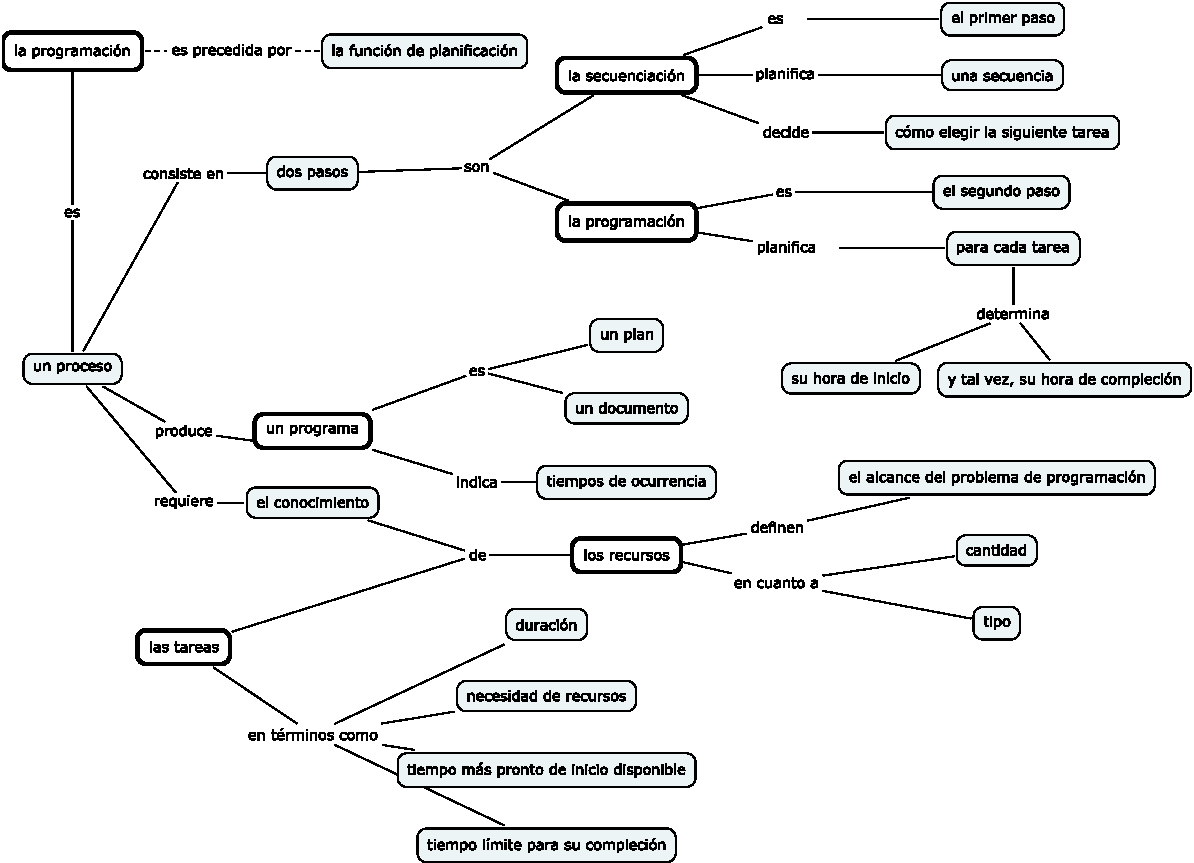
\includegraphics[width=\textheight]{scheduling.pdf}
\caption[La programación y sus elementos]{La programación y sus elementos}
\label{fig:programacion}
\end{sidewaysfigure}

\subsection{El proceso de programación} % (fold)
\label{proceso_programacion}

De acuerdo a \citet{wren95scheduling-timetabling}, el objetivo de la programación es solucionar problemas prácticos relacionados a la asignación, sujeta a restricciones, de recursos a objetos siendo colocados en el espacio-tiempo, haciendo uso o desarrollando herramientas apropiadas. Los problemas con frecuencia buscarán la satisfacción de ciertos objetivos \citetext{p.~47}.

\citet{wren95scheduling-timetabling} prosigue mencionando que la programación\index{programación} puede ser vista como el acomodo de recursos dentro de un patrón\index{programación!patrón} en el tiempo o espacio de manera tal que algunos objetivos\index{objetivo} sean alcanzados –o se acerquen a ello– y que restricciones\index{restricción} existentes en la manera en que los recursos pueden ser acomodados sean satisfechas –o casi satisfechas–.
%
Los recursos pueden ser personas, vehículos, clases, exámenes, máquinas, trabajos en una fábrica, es decir, cualquier cosa que sea del interés del dueño del problema.
%
Con frecuencia la conformación de los recursos puede ser vista como parte del proceso de programación\index{programación!proceso}. Por ejemplo, las herramientras de trabajo en una fábrica pueden ser acomodadas por turnos de personal, los cuales deben ser agrupados en listas, esta formación de turnos puede ser vista como un proceso específico de programación dentro de un proceso más extenso \citetext{p.~48}. 

\begin{figure}[hbtp]
\centering
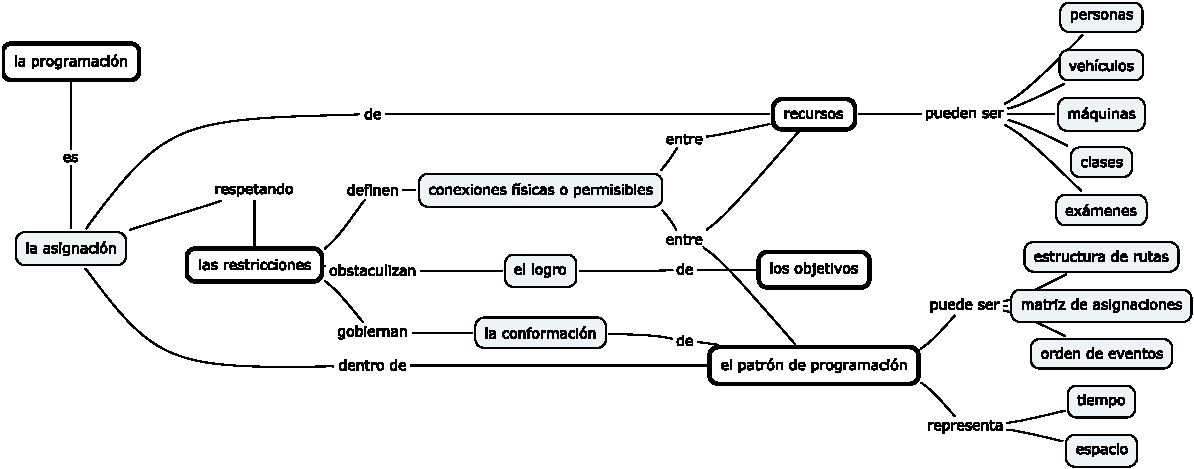
\includegraphics[width=\textwidth]{media/scheduling_process.pdf}
\caption[El proceso de programación]{El proceso de programación}
\label{fig:scheduling_process}
\end{figure}

El patrón de programación\index{programación!patrón} puede ser un orden de eventos, una estructura de rutas, una matriz de asignaciones, entre otros. El patrón general de programación puede tener que ser elaborado como parte del proceso de programación, o puede ser una plantilla\index{programación!plantilla} pre-existente característica del problema\index{programación!problema general} en cuestión \citep[p.~48]{wren95scheduling-timetabling}.

Las restricciones\index{restricción} definen conexiones físicas o permisibles entre los recursos\index{recurso}, y entre estos y el patrón\index{programación!patrón} de programación. Ellas gobiernan la manera en la cual los recursos pueden acomodarse juntos o dentro del patrón. Las restricciones pueden ser vistas como reglas que obstaculizan el logro de los objetivos\index{objetivo}. No obstante, también pueden ser vistas como parte de la especificación del problema\index{programación!problema general} siendo posible utilizarlas para guiar a la herramienta\index{programación!herramienta} de búsqueda de soluciones a una respuesta.
%
En la figura \ref{fig:scheduling_process} se presentan los conceptos ya descritos.
%
Algunas restricciones existen únicamente desde el punto de vista del dueño del problema, y pueden formar parte del proceso\index{programación!proceso} de solución con el propósito de mostrar hasta qué grado una solución podría ser mejorada si una restricción o restricciones fueran relajadas, de manera que el dueño pueda decidir si la restricción es realmente necesaria o si vale la pena hacer el esfuerzo de eliminarla de la definición del problema \citep[p.~48]{wren95scheduling-timetabling}.

\subsection{Programa, secuencia, horario}
\label{programa_secuencia_horario}

En ocasiones los términos programa\index{programa} (\textit{schedule}), secuencia\index{secuencia} (\textit{sequence}) y horario\index{horario} (\textit{timetable}) son utilizados a la ligera como si fueran sinónimos. Aquí se presentan algunas distinciones ajustándose a las prácticas aceptadas y procurando mantener tanta coherencia como sea posible \citep[p.~48]{wren95scheduling-timetabling}.

Un \textbf{horario}\index{horario} muestra cuándo deben ocurrir eventos\index{evento} particulares. No necesariamente implica una asignación\index{asignación} de recursos\index{recursos}. Por ende, un horario publicado de trenes o autobuses muestra cuándo deben ocurrir las salidas para una o más rutas distintas, sin embargo, no nos dice cuáles vehículos o conductores han de ser asignados a trayectos en específico.
%
La asignación de vehículos y conductores es parte del proceso\index{programación!proceso} de programación. Aunque la calendarización\index{calendarización} (\textit{timetabling}) –la acción de producir horarios– es estrictamente el diseño del patrón\index{programación!patrón} de trayectos, este patrón puede ser concebido como parte de un proceso que toma en consideración si es probable que un programa\index{programa} eficiente pueda ser ajustado al patrón de trayectos resultante \cite[p.~48]{wren95scheduling-timetabling}.

En el ámbito ferroviario, el término calendarización\index{calendarización} es utilizado con frecuencia para referirse a la construcción de una ruta –con tiempos– para un tren a través de un sistema. Siendo así que el «Escocés Volador» –mundialmente famoso tren de pasajeros exprés que recorre desde 1862 el trayecto Londres-Edinburgo– solía partir de Edinburgo (estación \textit{Waverly}) a las 10:00; el trabajo de calendarización era el proceso de la búsqueda de tiempos y rutas a través del sistema de trenes que no conflictuaran con otro tráfico –haciendo revisiones en el resto del tráfico de ser necesario– hasta que llegaba a Londres (estación \textit{Kings Cross}) a las 18:30 (en 1922) o 18:05 (1948) 
\citep[p.~48, 49]{wren95scheduling-timetabling}.

Un horario\index{horario!educacional} educacional también muestra cuándo deben ocurrir eventos en particular. En ciertas circunstancias puede no haber actividad de programación\index{programación} necesaria para producir tal horario\index{horario}. En una escuela donde un único maestro es el responsable por todas las actividades\index{actividad} de una clase\index{clase} en particular, y donde dichas actividades\index{actividad} ocurren en un mismo lugar, un horario\index{horario} no es más que una declaración respecto a los tiempos en que deberán ocurrir actividades específicas –como en el caso del «Escocés Volador»–.
%
En contraste, un horario de exámenes para una universidad normalmente incluirá la asignación de aulas elaboradas a partir del conocimiento del tamaño de los grupos y de las instalaciones especiales requeridas. Habrá sido conformado sujeto a restricciones duras\index{restricción!dura} y suaves\index{restricción!suave}, como la cantidad de exámenes que puede presentar un estudiante en periodos consecutivos. Un horario de cursos para una universidad también tiene que tomar en cuenta la disponibilidad de los conferenciantes individualmente.
%
Es por ello que las actividades de calendarización de cursos\index{calendarización!de cursos} y calendarización de exámenes\index{calendarización!de exámenes} en universidades\index{horario!en universidades} pueder ser consideradas actividades\index{actividad} de programación\index{programación} \citep[p.~49]{wren95scheduling-timetabling}. 

\begin{sidewaysfigure}
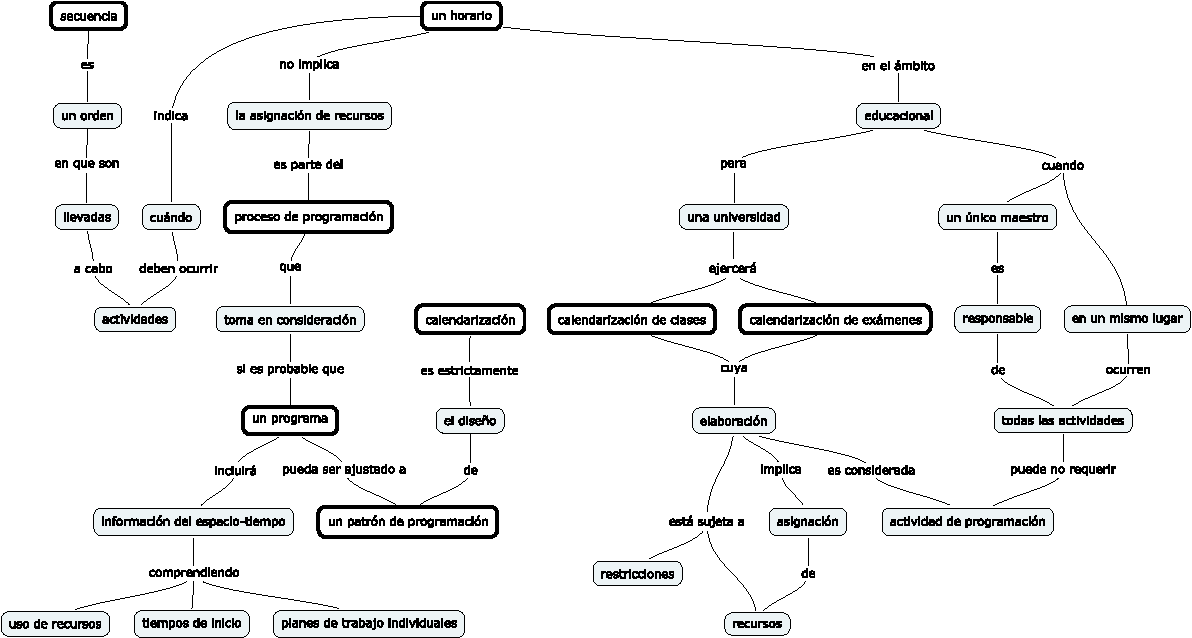
\includegraphics[width=\textwidth]{media/programa_secuencia_horario.pdf}
\caption[Programa, secuencia, horario]{Programa, secuencia, horario}
\label{fig:programa_secuencia_horario}
\end{sidewaysfigure}

Una \textbf{secuencia}\index{secuenciación!secuencia} es simplemente un orden en que las actividades\index{actividad} son llevadas a cabo. Por ejemplo, el orden en el que los trabajos son procesados a través de las máquinas en una fábrica, si los trabajos pasan a través de cada máquina en el mismo orden, es una secuencia. La secuenciación\index{secuenciación} puede tomar en cuenta costos relacionados a un trabajo específico siendo seguido por otro, como el costo de conversión de máquina. El problema de la secuenciación\index{secuenciación} de trabajos en estas circunstancias es conocido como un problema \textit{flow-shop}\index{secuenciación!flow-shop} \citep[p.~49]{wren95scheduling-timetabling}. 

Un \textbf{programa}\index{programa} normalmente incluirá toda la información espacial y temporal necesaria para que un proceso\index{proceso} llegue a término. Esto comprenderá los tiempos de inicio de las actividades\index{actividad} pertinentes, aserciones respecto a dónde serán asignados\index{asignación} cuáles recursos\index{recurso}, así como los planes de trabajo individuales para el personal o las máquinas.
%
Por consiguiente, la programación\index{programación} es el proceso\index{programación!proceso} de la elaboración del programa\index{programa}, incluyendo la asignación\index{asignación} de recursos\index{recurso} \citep[p.~49]{wren95scheduling-timetabling}.
%
En la figura \ref{fig:programa_secuencia_horario} se ilustran los conceptos anteriores.

\subsection{Definiciones}
\label{Definiciones}

Algunos autores consideran a la programación\index{programación} (\textit{scheduling}) y calendarización\index{calendarización} (\textit{timetabling}) como actividades distintas, en este trabajo se utilizará el término programación\index{programación} tanto como un término genérico y para cubrir tipos específicos de problemas, y se considerará a la calendarización\index{programación!calendarización} (\textit{timetabling}), secuenciación\index{programación!secuenciación} (\textit{sequencing}) y establecimiento de listas\index{programación!listas} (\textit{rostering}) como casos especiales de la actividad genérica de programación\index{programación} \citep[p.~47]{wren95scheduling-timetabling}.

En la sub-sección \ref{proceso_programacion} definimos el objetivo de la programación de acuerdo a \citet{wren95scheduling-timetabling} como:

\begin{quotation}
solucionar problemas prácticos relacionados a la asignación, sujeta a restricciones, de recursos a objetos siendo colocados en el espacio-tiempo, haciendo uso o desarrollando herramientas apropiadas. Los problemas con frecuencia buscarán la satisfacción de ciertos objetivos \citetext{p.~47}.
\end{quotation}

Para \citet{wren95scheduling-timetabling}, las actividades de calendarización\index{programación!calendarización}, establecimiento de listas\index{programación!listas} y secuenciación\index{programación!secuenciación} todas se apegan a la definición anterior \citetext{p.~53}.
%
Sin embargo, se hará uso de las siguientes definiciones más restrictivas para este trabajo.

\begin{quotation}
La \textbf{programación} es la asignación, sujeta a restricciones, de recursos a objetos siendo colocados en el espacio-tiempo, de manera tal que se minimice el costo total de algún conjunto de los recursos usados. Ejemplos comunes son la programación de transporte o el diseño de rutas para vehículos de entrega que buscan minimizar el número de vehículos o conductores y dentro de ese mínimo minimizar el costo total, y la programación \textit{job-shop} que puede buscar minimizar el número de periodo de tiempos usados, o algún recurso físico.

La \textbf{calendarización} es la asignación, sujeta a restricciones, de recursos dados a objetos siendo colocados en el espacio-tiempo, de manera tal que se satisfaga tanto como sea posible un conjunto de objetivos deseados. De ejemplo están la calendarización de cursos y exámenes y algunas formas de asignación de personal, como la ocupación de puestos en casetas de cobro sujetas a un número limitado de personal.

La \textbf{secuenciación} es la construcción, sujeta a restricciones, de un orden en el que actividades deben ser llevadas a cabo u objetos que deben ser colocados en alguna representación de una solución. Como ejemplos están la programación \textit{flow-shop} y el problema del agente viajero.

El \textbf{establecimiento de listas} es la colocación, sujeta a restricciones, de recursos en espacios dentro de un patrón. Uno puede buscar minimizar algún objetivo, o simplemente lograr una asignación factible. Frecuentemente los recursos rotarán a través de una lista. \citetext{p.~53}
\end{quotation}

Algunos problemas pueden encajar en más de una de las deficiones anteriores, y los términos tienen a ser utilizados de manera holgada en el área de trabajo y en la comunidad de investigación del área.
%
En algunas se ha referido a la satisfacción o a la minimización. Debe ser resaltado que muchos de los problemas que se tratan en el área no tienen un objetivo bien definido. En ocasiones se puede justificar el uso de métodos de mejora o no-óptimos en parte porque los distintos dueños del problema tienen distintas perspectivas del objetivo, aunque en realidad tales métodos son frecuentemente utilizados simplemente porque no hay un método óptimo (o exacto) que sea viable en la práctica \citep[p.~53,~54]{wren95scheduling-timetabling}

\citet[p.~3]{Baker2009} recuerda que muchos de los primeros desarrollos en el campo de la programación fueron motivados por problemas encontrados en la industria de la producción. Por lo tanto, es natural encontrar en la literatura el uso de vocabulario de producción cuando se describen problemas de programación. Aún cuando hoy día la aplicación de la programación es de considerable importancia en múltiples áreas no relacionadas con la producción, la terminología sigue siendo frecuentemente utilizada. Es por eso que a los recursos usualmente se les llama \textbf{máquinas} (\textit{machines}) y a las tareas se les llaman \textbf{trabajos} (\textit{jobs}). En ocasiones, los trabajos pueden consistir de varias tareas elementales llamadas \textbf{operaciones} (\textit{operations}). El ambiente del problema de programación es llamado el \textbf{taller de trabajo} (\textit{job-shop}), o simplemente, el \textbf{taller} (\textit{shop}). Por ejemplo, un problema de programación que trate con el procesamiento de pólizas de seguros en aseguradoras puede ser descrito de manera genérica como un «taller» de seguros que se encarga del procesamiento de «trabajos» de polizas por «máquinas» aseguradoras.

\section{Historia}
\label{historia_programación}

El concepto de programación no es nuevo; las pirámides tienen más de 3,000 años, Sun Tzu escribió acerca de programación y estrategia desde una perspectiva militar hace 2,500 años, vías ferroviarias han sido construidas por alrededor de 200 años, entre otros muchos ejemplos. Ninguna de estas actividades pudo haber sido lograda sin alguna forma de programación –como lo es el entendimiento de conceptos como actividad y secuenciación–. Sin embargo, mientras que los administradores, sacerdotes y líderes militares en control de las organizaciones responsables por el logro de estas actividades debieron tener una apreciación por la programación –o al menos aquellos que tuvieron éxito– existe poca evidencia de procesos formales hasta la aparición del siglo XX \citep[p.~2]{Weaver2006}.

\begin{figure}[hbtp]
\centering
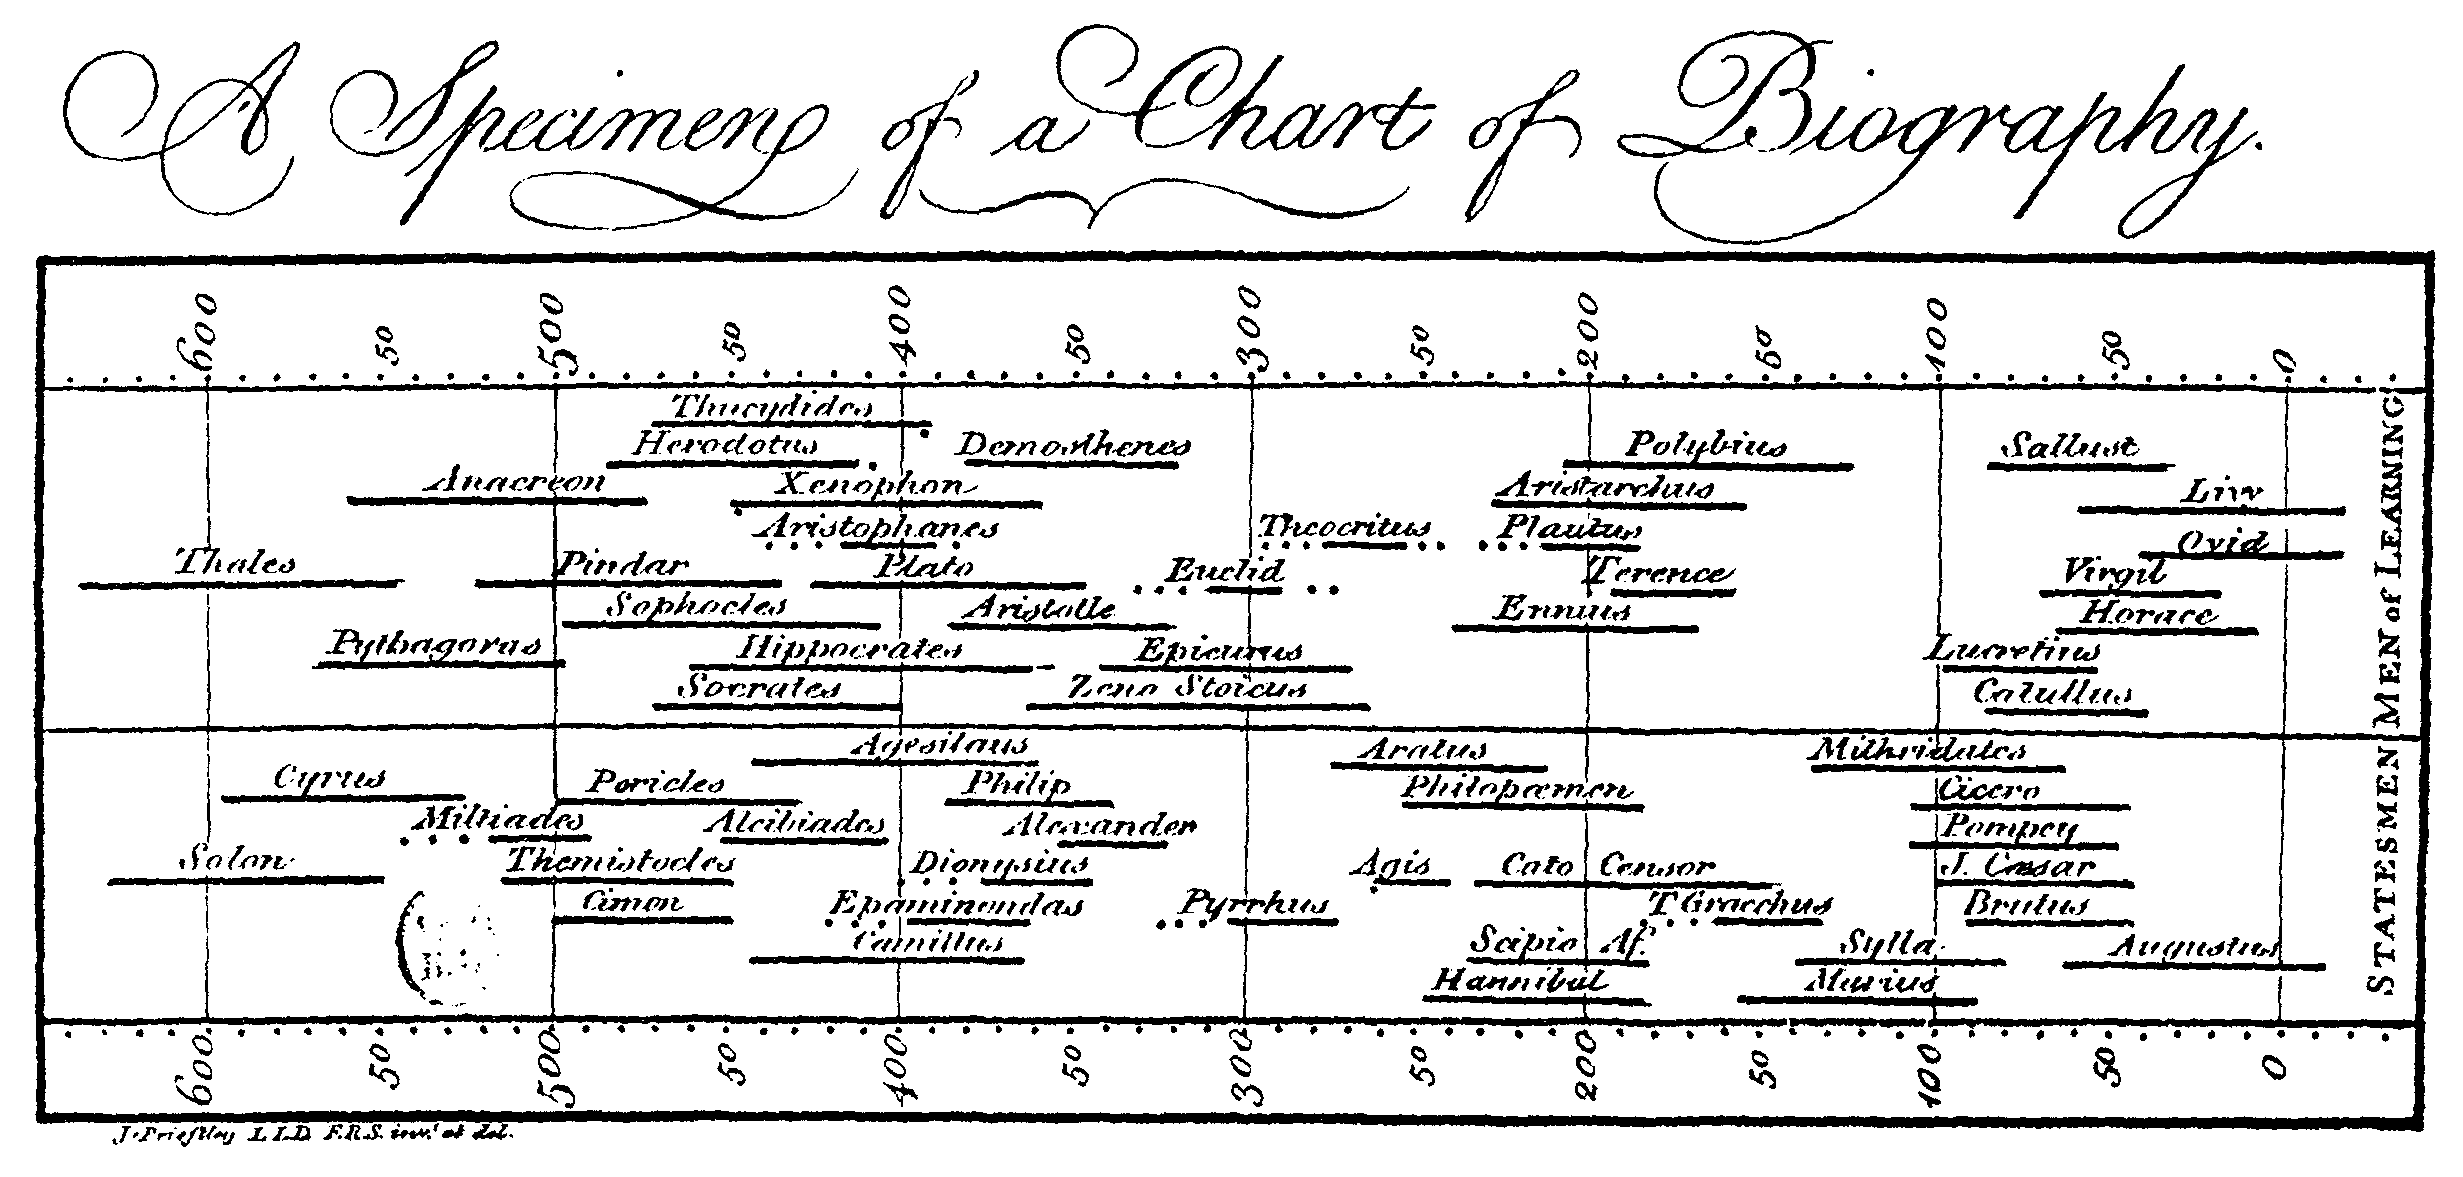
\includegraphics[width=\textwidth]{media/PriestleyChart.png}
\caption[Gr\'afica de Biograf\'ia]{Gr\'afica de Biograf\'ia abarcando los primeros 650 años antes de la era común. De \textit{A description of a chart of biography}, por J. \citeauthor{priestley1764description}, \citeyear{priestley1764description}. Derechos de autor expirados, obra del dominio público.}
\label{fig:chart_biography}
\end{figure}

De acuerdo a \citet{Weaver2006}, las herramientas de control de programación modernas pueden trazar sus orígenes hasta 1765. El creador de la gráfica de barra parece ser Joseph Priestley (Inglaterra, 1733-1804); su «Gráfica de Biografía» mostraba unos 2,000 lapsos de vida de personajes notables en una gráfica con escala de tiempo, véase la figura \ref{fig:chart_biography}. Las ideas de Priestley fueron retomadas por William Playfair (1759-1823) en su Atlas Comercial y Político (\textit{Commercial and Political Atlas}) de 1786. A Playfair se le atribuye el desarrollo de un vasto rango de gráficas incluyendo la línea, la barra (histograma), y las gráficas circulares (gráficas de pastel), un ejemplo puede ser visto en la figura \ref{fig:playfair_timeseries} \citetext{p.~2,~3}.

\begin{sidewaysfigure}
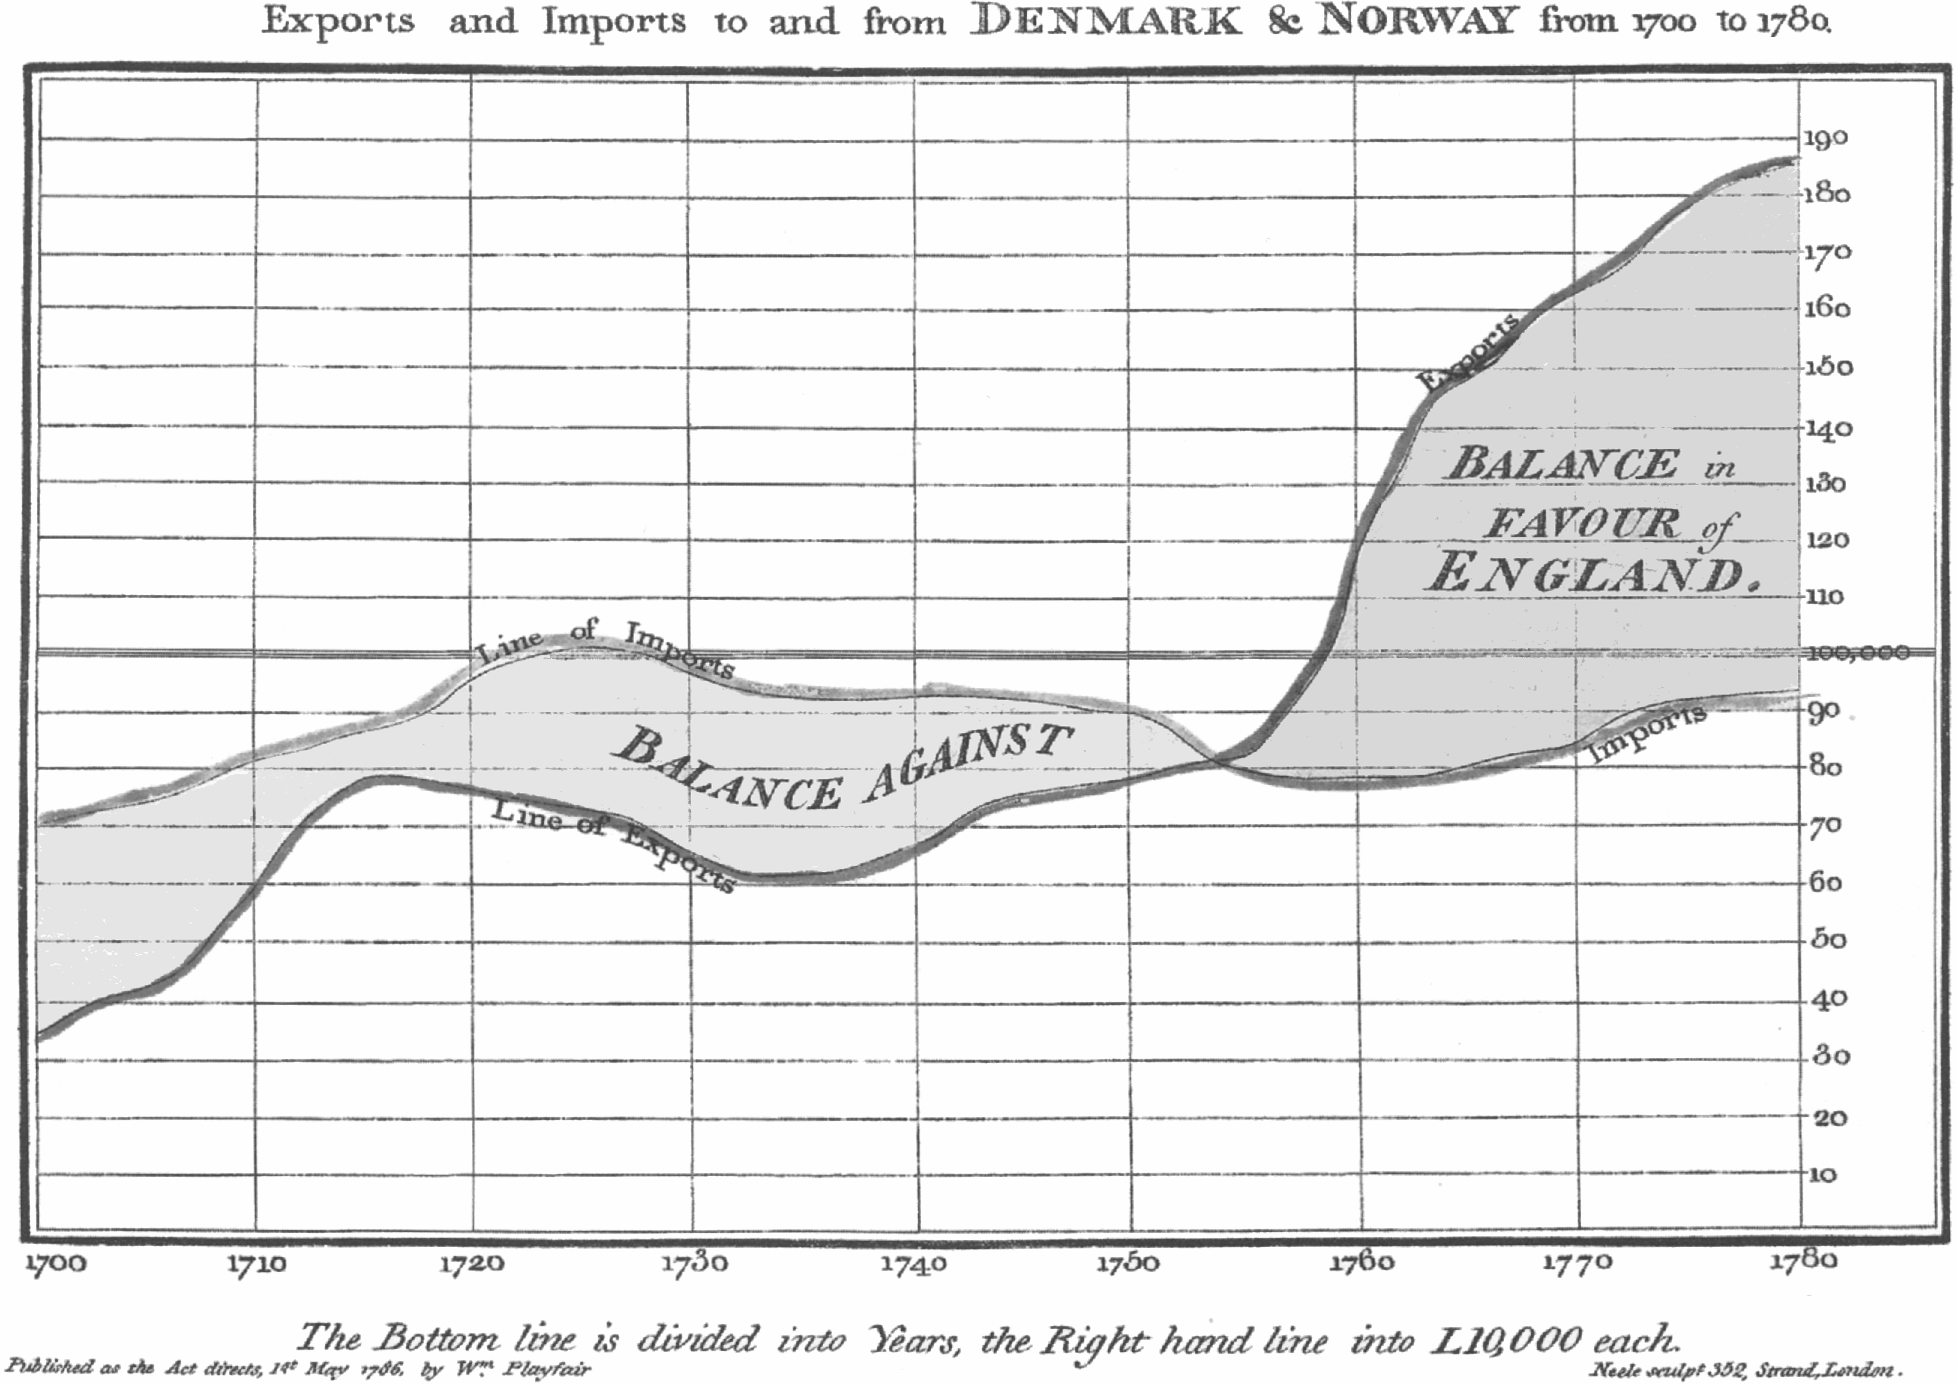
\includegraphics[width=\textwidth]{media/Playfair_TimeSeries.png}
\caption[Gráfica del Atlas de W. Playfair]{Una de las gráficas elaboradas por Playfair. De \textit{The Commercial and Political Atlas}, por W. \citeauthor{playfair1786commercial}, \citeyear{playfair1786commercial}. Derechos de autor expirados, obra del dominio público.}
\label{fig:playfair_timeseries}
\end{sidewaysfigure}

Siguiendo los pasos de Playfair, Karol Adamiecki –un polaco economista, ingeniero e investigador de la administración– desarrolló el harmonograma en 1896. Este gráfico dispone de una escala de tiempo en el eje  vertical (del lado izquierdo) y enumera las actividades en la parte superior. La hora de inicio y la duración de las actividades se muestra por una «barra deslizante» (muy similar a la «barra» en una gráfica de barra). Lo relevante del harmonograma es que también tabula cada actividad predecesora y sucesora haciéndolo un predecesor distinto de los sistemas CPM y PERT desarrollados uons 60 años después \citep[p.~3]{Weaver2006}.

Para 1912, la gráfica de barras moderna aparenta estar totalmente desarrollada y es utilizada al menos en Alemania. Estas ideas fueron entonces publicitadas en EE.UU. por el consultor de administración estadounidense Henry L. Gantt, quien publicó Trabajo, Sueldos y Utilidades (\textit{Work, Wages, and Profits}) en 1916 en donde expresamente habla de la programación, especialmente en el ambiente de los talleres de trabajo. En su forma más pura, la gráfica de barras correlaciona actividades y tiempos en una presentación gráfica permitiendo la determinación de la temporización del trabajo pero no de sus interdependencias. Como se muestra en la figura \ref{fig:grafica_gantt}, la secuenciación es inferida en lugar de ser mostrada y en sus elaboraciones hechas a mano, las primeras gráficas eran una representación estática del programa \citep[p.~3]{Weaver2006}.

\begin{sidewaysfigure}
\centering
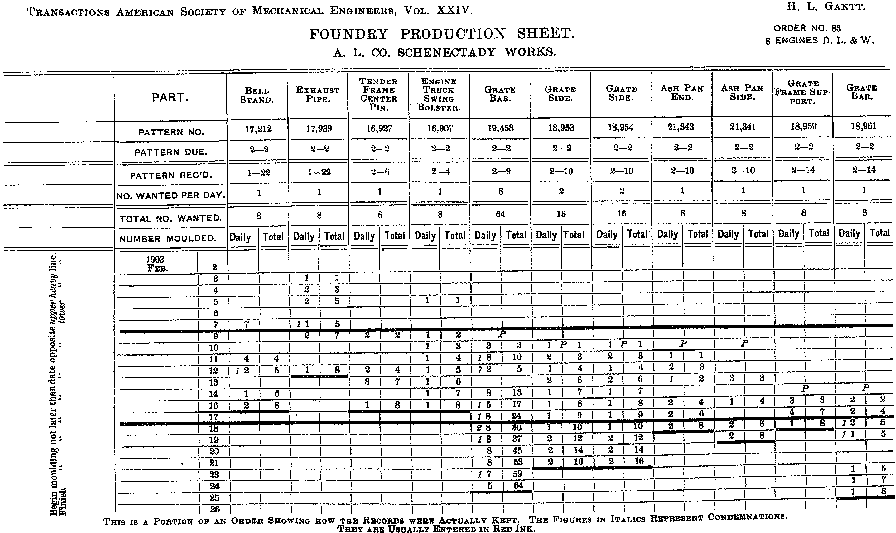
\includegraphics[width=\textwidth]{media/gantt-graphic.pdf}
\caption[Gráfica de Gantt]{Gráfica de Gantt. De \textit{Gantt charts: A centenary appreciation}, por J. M. \citeauthor{wilson2003gantt}, \citeyear{wilson2003gantt}, \textit{European Journal of Operational Research}, 149, p.~2. Derechos reservados [\citeyear{wilson2003gantt}] por \textit{European Journal of Operational Research}.}
\label{fig:grafica_gantt}
\end{sidewaysfigure}

La planeación de líneas de flujo (\textit{flowline planning}) fue desarrollada en la década de los treinta o aún antes y las gráficas de Milestone tambien estuvieron en uso regular para la decada de los cincuenta. Grandes contratos eran subdivididos en secciones con fechas límite para la compleción del trabajo necesario para alcanzar las metas de cada hito (\textit{milestone}). Sin embargo, así como con las graficas de Gantt, todas las fechas y las relaciones mostradas en estas graficas estaban basadas en heuristicos o en experiencia. Era posible identificar retrasos pero cualquier valoración del impacto del mismo estaba basada en un punto de vista personal de los datos y no de un analisis serio. Como consecuencia cuando el retraso de un programa se volvia aparente en grandes contratos, la tendencia era solucionar el problema inundandolo con mano de obra y «comprar tiempo» frecuentemente a un precio muy elevado \citep[p.~4]{Weaver2006}.

Independiente del desarrollo de los procesos de control de programacion basados en graficas de barras y en milestones, el programacion lineal habia estado siendo investigado por varios años. Esta rama de las matematicas miraba en la causa y efecto de las acciones entre ellas en situaciones tales como el flujo de trafico en una autopista. Uno los matematicos involucrados en ese trabajo fue James E. Kelley \citep[p.~4]{Weaver2006}.

La evolución de la programación siguió de cerca el desarrollo de las computadoras. Los primeros sistemas eran computadoras centrales gigantescas, típicamente le tomaba a un nuevo programador muchos meses aprender a utilizarlas. Estos sistemas migraron a las mini-computadoras de la década de los setenta y ochenta pero continuaron siendo onerosos, fomentando así el uso generalizado de técnicas manuales de programación, solo las organizaciones más grandes –o más sofisticadas– pudieron sufragar una oficina central de programación y los sistemas de cómputo necesarios \citep[p.~2]{Weaver2006}.

El advenimiento de la micro-computadora –entiéndase la PC o computadora personal– cambió la programación para siempre. La evolución de la programación basada en tecnología PC cambió los controles del proyecto de un ambiente en donde un equipo especializado de programadores operaba sistemas costosos asegurándose que la programación era orrecta –y que la organización tenía el control de los datos– a una situación en donde cualquiera podía aprender a manejar un paquete de software de programación, los programas se convirtieron en islas de información dispersas en los escritorios de los empleados y la calidad de la programación en general se desplomó \citep[p.~2]{Weaver2006}.

En la actualidad, hay tendencias de un regreso a los sistemas empresariales soportados por paquetes Ofimáticos de Administración de Proyectos (\textit{Project Management Office; PMO}) que corrigen el balance y ofrecen lo mejor de los dos mundos. Desde un punto de vista tecnológico, la información es gestionada de manera central, pero está disponible fácilmente para todos en cualquier PC a través de una interfaz de red. Desde el punto de vista de habilidades, los \textit{PMO} están teniendo un impacto en el desarrollo de las carreras de los programadores y apoyando en la implementación de estándares de programación dentro de las organizaciones \citep[p.~2]{Weaver2006}.

\subsection{Reseña de problemas clásicos}
\label{resena_problemas_clasicos}

\section{Áreas de aplicación}
\label{areas_aplicacion}

Los problemas de programación se encuentran en todos los niveles y en todos los sectores de la actividad económica. Generalmente, se hace una distinción entre aquellos relacionados a la industria de la fabricación y aquellos relacionados a los sistemas de cómputo o administración de proyectos \citep[p.~6]{TKindt2002}.

\subsection{Problemas relacionados a la producción} % (fold)
\label{problemas_relacionados_produccion}

Los problemas de programación se encuentran en los sistemas de manufactura flexible (\textit{FMS; Flexible Manufacturing System}). Numerosas definiciones de un \textit{FMS} existen en la literatura. Para Liu y MacCarthy (1996), «un FMS comprende tres elementos principales: herramientas de maquinaria controladas por computadora; un sistema de transporte automatizado y un sistema de control por computadora» (como está citado en \citealp[p.~6]{TKindt2002})  Estos problemas son tratados en la literatura y seguido en una bien definida clase de aplicación. Además, este amplio problema abarca otros problemas relacionados con la \textbf{Programación de Celdas Robotizadas} y la \textbf{Programación de Vehículos Guiados Automatizados}.

Igualmente, la \textbf{electrodeposición} y los \textbf{talleres químicos} tienen sus propias peculiaridades en los problemas de programación. El último también es conocido como Problemas de Programación de Grúas. Estos talleres se caracterizan por la presencia de una o más grúas compartiendo el mismo espacio físico y donde deben transportar productos para tratamientos en tanques. Por lo general, el tiempo de submersión en un tanque está limitado por un mínimo y un máximo –el intervalo del tiempo de procesamiento–, el tiempo de transporte no es despreciable y las operaciones deben ser llevadas a cabo sin tiempos de espera. Estos problemas son muy comunes en la industra y los casos simples –mono-robot, tanques de una pasada, etc.– ya tienen planteadas buenas soluciones \citep[p.~6,~7]{TKindt2002}.


\section{Teoría de la programación}
\label{teoria_programacion}

De acuerdo a \citet[p.~1]{TKindt2002}, la teoría de la programación aparece a mediados de la década de los cincuenta. Desde entonces los problemas planteados se han acercado cada vez más a aplicaciones industriales y de esta manera se han incrementado en complejidad. La disposición de las máquinas se asemejan más y más a lo encontrado en la práctica. Al mismo tiempo las restricciones impuestas son cada vez más concretas.  Paradójicamente, la literatura muestra que en la mayoría de los problemas planteados, los programas son evaluados por un único criterio. 

Durante las diferentes etapas de planificación distintos criterios pueden ser considerados. A un nivel estratégico, una planificación de largo alcance puede contemplar varios años, los objetivos se preocupan con la minimización de costos relacionados a los planes de inversión para materiales, finanzas, o personal, relacionados a la elección de nuevas oportunidades de negocio, o al lanzamiento de campañas de publicidad. Para la planificación estratégica en una fase de mediano plazo con varios meses en mente, los objetivos se enfocan a la minimización de costos: costos de inventario, costos de transporte de insumos, costos de modificación en la capacidad de producción, costos de lanzamiento, costos de modificación de sistemas de producción entre otros. Durante una fase de planificación o una fase de programación a corto plazo –un periodo de tiempo de una semana– multiples objetivos requieren la atención del ejecutivo de producción: ante todo, debe considerar los retrasos para la satisfacción del cliente, acto seguido, debe minimizar el costo del trabajo en proceso de la producción, y finalmente debe minimizar los costos de producción relacionados al tiempo utilizado para la configuraciónd de la maquinaria o los tiempos muertos de las mismas. Es por ello, que un problema de programación puede contemplar multiples criterios de manera tal que permita ofrecer al dueño del problema soluciones más realistas\citep[p.~1]{TKindt2002}.

ésta se preocupa primariamente con modelos matemáticos que se relacionan al proceso de programación. El desarrollo de modelos útiles, los cuales derivan en técnicas de solución y perspectivas prácticas, han sido la interfaz continua entre la teoría y la práctica. 
%
La perspectiva teorética es en gran medida un acercamiento cuantitativo, uno que intenta capturar la estructura del problema de una manera matemática.
%
En particular, este enfoque cuantitativo comiento con la descripción de los recursos y tareas, y con la traducción de objetivos de planificación en una \textbf{función objetivo} explícita.

Idealmente, la función objetivo debe consistir de todos los costos que dependan de decisiones de programación. En la práctica, sin embargo, tales costos son frecuentemente difíciles de medir, o incluso de identificar en su totalidad. Los costos de operación mayores –y los más inmediatamente identificables– son determinados por la \textbf{función de planificación}, mientras que los costos relacionados con la programación son difíciles de aislar y frecuentemente tienden a dar la impresión de ser costos fijos.


\subsection{Teoría de la complejidad computacional} % (fold)
\label{teoria_complejidad_computacional}

Una perspectiva útil en cuanto a la relación de los problemas de programación y sus técnicas de solución viene de los avances de una rama de la ciencia computacional conocida como \textbf{teoría de la complejidad computacional}. La noción de la complejidad se refiere al esfuerzo computacional requerido por un algoritmo de solución. El esfuerzo de computación es descrito con una notación de orden de magnitud.
%
Por ejemplo, se hace uso de un algoritmo en particular para resolver un problema de tamaño \textit{n}. (Técnicamente, \textit{n} denota la cantidad de información necesaria para especificar el problema.) El número de computaciones requeridas por el algoritmo típicamente está vinculado desde encima por una función de \textit{n}. Si la orden de magnitud de esta función es polinomial conforme \textit{n} se agranda, entonces decimos que el algoritmo es polinomial.
%
Por ejemplo, si la función tiene una orden de magnitud $\textit{n}^2$, denotada por $\BigO(\textit{n}^2)$ entonces el algoritmo es polinomial. Por otra parte, si la función es $\BigO(2^\textit{n})$, entonces el algoritmo es no-polinomial (en este caso sería exponencial). Siendo todo lo demás igual, son preferibles los algoritmos polinomiales puesto que conforme \textit{n} se agranda, estos son ultimadamente más rápidos.

\chapter{Una visión general del problema}
\label{vision_general_problema}

\section{Introducción}
\label{introduccion_vision_general}

En las secciones \ref{calendarizacion_clases}, \ref{calendarizacion_cursos} y \ref{calendarizacion_examenes} se presentan de manera general las formulaciones formales de los problemas.
La sección \ref{problema_general_programacion_horarios} presenta el problema general de la programación de horarios\index{programación!problema general}. La sección \ref{clasificacion_problemas} presenta una clasificación\index{calendarización!clasificación} de los tipos de problemas encontrados en la programación de horarios educacionales. 
\section{El problema general de la programación de horarios}
\label{problema_general_programacion_horarios}

\index{horarios!programación!problema general}
\citet[p.~53]{wren95scheduling-timetabling} definió la programación de horarios como “la asignación, sujeta a restricciones\index{restricción}, de recursos\index{recurso} dados a objetos siendo acomodados en un espacio-tiempo, de tal manera que se satisfagan tanto como sea posible un conjunto de objetivos deseados.”

\iffalse
Timetabling is the allocation, subject to constraints, of given resources to objects being placed in space-time, in such a way as to satisfy as nearly as possible a set of desirable objectives. Examples are class and examination timetabling and some forms of personnel allocation, for example manning of toll booths subject to a given number of personnel.

“Timetabling is the allocation, subject to constraints, of given resources to objects being placed in space time, in such a way as to satisfy as nearly as possible a set of desirable objectives.”
\fi

\section{Calendarización educacional} % (fold)
\label{calendarizacion_educacional}


\section{Clasificación de los problemas en el ámbito educacional}
\label{clasificacion_problemas}

\index{clasificación}
El problema de la programación de horarios educacionales\index{horarios!educacionales} se clasifica en tres clases principalmente:
calendarización de clases\index{horarios!de clases} (\textit{school timetabling}),
calendarización de cursos\index{calendarización!de cursos} (\textit{course timetabling}) y
calendarización de exámenes\index{calendarización!de exámenes} (\textit{examination timetabling}) \citep[p.~88]{schaerf99a-survey-of-automated}.

Todos tienen en común las características básicas del problema general de programación de horarios\index{horarios!problema general} pero pueden presentar diferencias significativas entre ellos. Cada problema cuenta con su propias restricciones\index{restricción}, requerimientos\index{requerimiento} y reglas\index{regla}. Son agrupados por su ámbito de aplicación en horarios en escuelas\index{horarios!en escuelas} y horarios en universidades\index{horarios!en universidades} \citep[p.~10]{abdullah06heuristic-approaches}.

\begin{figure}[hbtp]
\centering
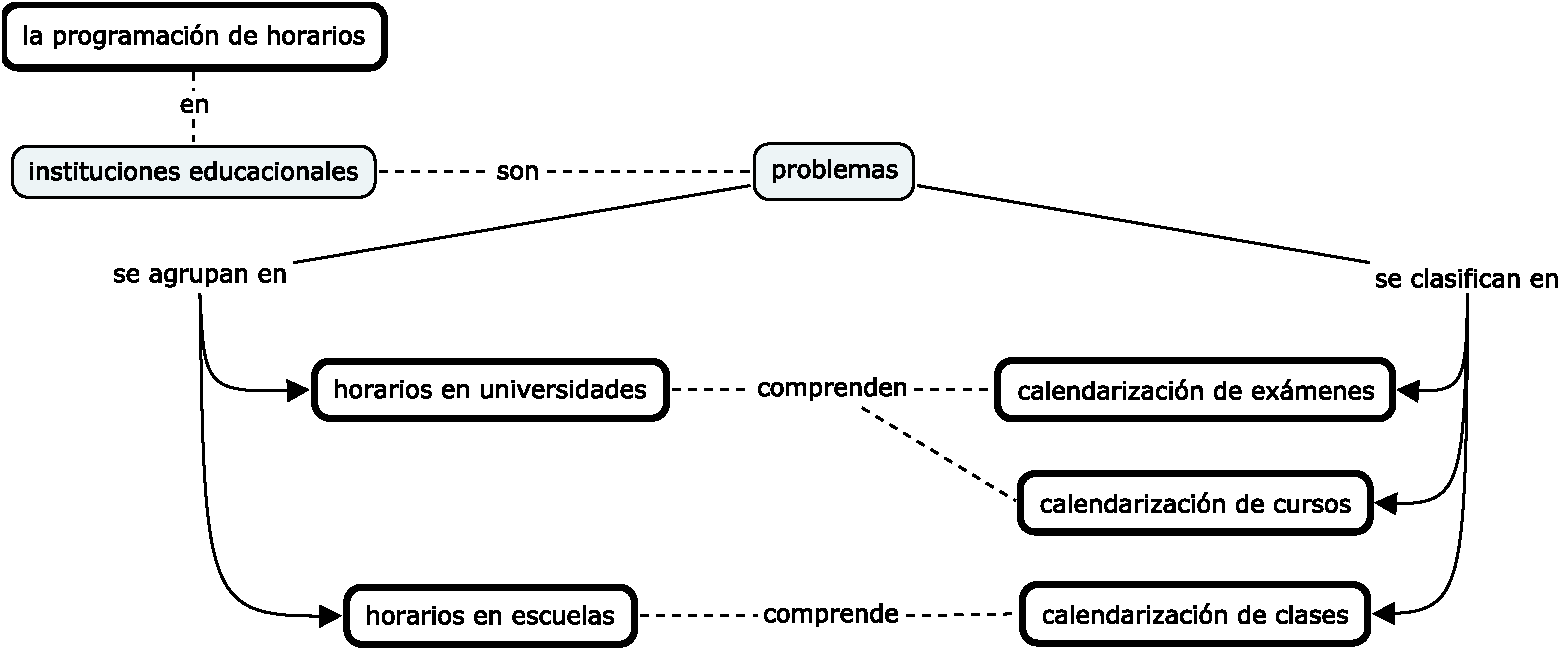
\includegraphics[width=\textwidth]{timetabling_classification.pdf}
\caption[Clasificación del problema]{Clasificación de los problemas en la elaboración de horarios educacionales}
\label{fig:timetabling_classification}
\end{figure}

\iffalse
Classification of Educational Timetabling Problems
Schaerf (1999a) classified educational timetabling into three main classes i.e. school timetabling, course timetabling and examination timetabling. They share the same basic characteristics of the general timetabling problem but can still have significant differences between them. Each one of them has its own constraints, requirements and rules. More details on educational timetabling can be found in Burke et al. (2004e). In this section, a classification of educational timetabling and its properties are discussed. We divided educational timetabling into two categories i.e. school timetabling and university timetabling (which consists of examination timetabling and course timetabling).
\fi

\subsection{Horarios en escuelas}

\index{horarios!en escuelas}

\subsubsection{Horarios de clases}

\index{horarios!de clases}
De acuerdo a \citet[p.~88]{schaerf99a-survey-of-automated} el problema de horarios de clases consiste en calendarizar en un periodo semanal todas las clases de una escuela, evitando que los profesores se encuentren con dos clases al mismo tiempo, y viceversa. \citet[p.~10,11]{abdullah06heuristic-approaches} elabora explicando que el problema consiste de un conjunto de profesores, clases, lecciones y periodos semanales. En donde tales periodos semanales son predefinidos.

El problema intenta asignar lecciones a periodos y, un profesor a una clase en particular en un momento dado mientras se satisface un conjunto de limitaciones con el fin producir un horario factible. Algunos ejemplos de limitaciones en este tipo de problemas son las capacidades de alojamiento, ubicaciones, cargas de trabajo de los profesores, tiempo de descanso entre lecciones.

\subsection{Horarios en universidades}

\index{horarios!en universidades}\index{calendarización!de cursos}\index{calendarización!de exámenes}
El problema de la planificación de horarios en universidades puede ser agrupado en dos categorías: (i) calendarización de cursos y (ii) calendarización exámenes.
El problema de la calendarización de cursos es el proceso de la asignación de periodos y aulas de manera tal que las reuniones entre conferenciantes y estudiantes pueda ocurrir.
El problema de la calendarización de exámenes se refiere a la asignación de periodos y aulas de manera tal que los estudiantes puedan presentar sus exámenes.
Ambos problemas son similares de manera superficial, pero existen diferencias importantes que los distinguen.
En la calendarización de exámenes, múltiples exámenes pueden ser presentados en una misma aula (ej. auditorio) al mismo tiempo.
Sin embargo, esto no es posible para la calendarización de cursos en donde únicamente un curso puede ser asignado a un aula \citep[p.~11]{abdullah06heuristic-approaches}.

\subsubsection{Calendarización de exámenes}

\index{calendarización!de exámenes}\index{calendarización!de cursos}
\citet[p.~4]{carter95recent-developments} definió el problema como la asignación de exámenes a un número limitado de periodos de manera tal que no existan conflictos o coincidencias. Los problemas de calendarización de cursos y exámenes son similares pero algunas diferencias relevantes según \citet[p.~159]{werra85an-introduction-to-timetabling} son:
\begin{enumerate}[a]
\item Existe generalmente un solo exámen por cada tema (mientras que hay varias exposiciones en un curso)
\item En la calendarización semanal de cursos, el objetivo principal es evitar conflictos (ej. la ocurrencia de que dos cursos elegidos por un mismo estudiante sean programados en el mismo periodo). Para los exámenes, generalmente se pide un máximo de un examen por día para cada estudiante o de ser posible, evitar la calendarización de exámenes en días consecutivos si el periodo de evaluación de exámenes lo permite.
\end{enumerate}
El problema de la calendarización de exámenes es muy común tanto en escuelas como en universidades. La asignación de los exámenes a los periodos está sujeta a un conjunto de limitaciones \citep[p.~12]{abdullah06heuristic-approaches}.

\subsubsection{Calendarización de cursos}

\index{calendarización!de cursos}
El problema de la calendarización de cursos surge cuando una universidad (o incluso una escuela) ofrece una colección de cursos (cada uno consistiendo de un número dado de conferencias) sin existir un currículo fijo y en donde cada estudiante puede elegir cierto número de cursos. El problema consiste en la asignación de cada lectura a algún periodo en la semana de manera tal que ningún estudiante requiera asistir a más de una conferencia a la vez \citep[p.~157]{werra85an-introduction-to-timetabling}.
\citet[p.~88]{schaerf99a-survey-of-automated} define el problema como la calendarización semanal de todas las lecciones de un conjunto de cursos universitarios, minimizando los empalmes de las lecciones de cursos teniendo estudiantes en común.

\section{Calendarización de clases}
\label{calendarizacion_clases}

\section{Calendarización de cursos}
\label{calendarizacion_cursos}

\section{Calendarización de exámenes}
\label{calendarizacion_examenes}

\chapter{Modelos matemáticos}

\section{Introducción}

\section{planificación de horarios en escuelas}

\section{Calendarización de cursos}

\section{Calendarización de exámenes}

\section{Un lenguaje en común}

\section{Algoritmos de solución}

\chapter{Restricciones y funciones objetivo}

\section{Introducción}

\section{Restricciones}

\section{Funciones objetivo}

\chapter{El gestor escolar}

\section{Aplicaciones}

\subsection{Métricas de desempeño}

\subsection{Multidisciplinario}

\section{Factores de interés}

\subsection{Laborales}

\subsubsection{Regulatorios}

\subsection{Diagnóstico}

\subsubsection{Interinstitucional}

\subsection{Inversión}

\subsubsection{Downsizing}

\subsection{Económicos}

\subsubsection{Utilidades}

\subsubsection{Fiscales}

\subsubsection{Aprovechamiento de recursos}

\subsection{Sociales}

\subsubsection{Involucramiento de paterfamilias}

\subsection{Institucionales}

\subsubsection{Profesorado}

\subsection{Flexibilidad}

\chapter{Trabajo en el futuro y conclusiones}

\section{Resumen del trabajo de investigación}

\section{Contribuciones}

\section{Trabajo futuro}

\section{Diseminación}

\index{timetabling!university|see{programación de horarios en universidades}}
\index{timetabling!school|see{calendarización de clases y programación de horarios en escuelas}}
\index{timetabling!course|see{calendarización de cursos}}
\index{timetabling!examination|see{calendarización de exámenes}}

\index{scheduling|see{programación}}
\index{timetabling|see{calendarización}}

\index{schedule|see{programa}}
\index{sequence|see{secuencia}}
\index{timetable|see{horario}}

% Bibliography
\bibliographystyle{apalike}
\bibliography{/Users/harciga/Dropbox/bibliographies/reviewed,/Users/harciga/Dropbox/bibliographies/Dissertation_books}
{
\RaggedRight
\printindex
}
\end{document}
